\documentclass{beamer}
\usetheme{Madrid}

\usepackage{amsmath, amssymb, amsthm}
\usepackage{graphicx}
\usepackage{listings}
\usepackage{gensymb}
\usepackage{minted}
\usemintedstyle{friendly}
\definecolor{bg}{rgb}{0.95,0.95,0.95}
\usepackage[utf8]{inputenc}
\usepackage{hyperref}
\usepackage{gvv}
\begin{document}
\title{NCERT 9.4.3}
\author{EE24BTECH11032 - JOHN BOBBY}
\date{}
\frame{\titlepage}
\begin{frame}{Question}
    Find the solution of the differential equation $\frac{dy}{dx}=1-y$, using the trapezoidal method.Assume $y\brak{0}=0$
\end{frame}
\begin{frame}{Trapezoidal Rule}
\begin{align}
    \int_{a}^{b} f\brak{x}dx \approx \brak{b-a}\brak{\frac{f\brak{a}+f\brak{b}}{2}}\\
f\brak{y}=1-y=\frac{dy}{dx}
\end{align}
Integrating the equation $\brak{2}$ from $n$ to $n+1$
\begin{align}
    A=A_{n+1}-A_n&=\brak{x_{n+1}-x_n}\brak{\frac{f\brak{y_{n+1}}+f\brak{y_n}}{2}}\\
    A_{n+1}-A_n&=\brak{x_{n+1}-x_n}\brak{1-y_{n+1}+1-y_n}\\
    x_{n+1}-x_n&=h\\
    A_{n+1}-A_n&=h\brak{2-y_{n+1}-y_n}
\end{align}
On rearranging we get the difference equation,
\begin{align}
    y_{n+1}&=y_n+\frac{2-h}{2+h}y_n+\frac{2h}{2+h}
\end{align}
\end{frame}
\begin{frame}{Laplace Transform}
\begin{align}
    \mathcal{L}\brak{\frac{dy}{dx}} &= \mathcal{L}\brak{1 - y}
\end{align}
    $\mathcal{L}\brak{\frac{dy}{dx}} = sY(s) - y(0), \quad \mathcal{L}\brak{1} = \frac{1}{s}, \quad \mathcal{L}\brak{y(t)} = Y(s)$
\begin{align}
     sY(s) - y(0) = \frac{1}{s} - Y(s)\\
    sY(s) + Y(s) = \frac{1}{s} + y(0)\\
    Y(s)(s + 1) = \frac{1}{s} + y(0)\\
     Y(s) = \frac{1}{s(s+1)}
\end{align}


    
\end{frame}
\begin{frame}{Laplace Transform}
     Taking inverse Laplace Transform,
 \begin{align}
     \mathcal{L}^{-1}\brak{Y\brak{s}}=y\brak{x}\\
    \mathcal{L}^{-1}\brak{\frac{1}{s\brak{s+1}}}=1-e^{-x}\\
    y\brak{x}=1-e^{-x}
 \end{align}
\end{frame}
\begin{frame}{Bilinear Transform}
Let the laplace transform of $f\brak{y}=1-y$ be $X\brak{s}$
\begin{align}
    X\brak{s}=\mathcal{L}\brak{f\brak{x,y}}
\end{align}
Applying laplace transform on both sides of equation 
\begin{align}
    sY\brak{s}=X\brak{s}
\end{align}
Let $H\brak{s}$ be defined such that
\begin{align}
    H\brak{s}=\frac{Y\brak{s}}{X\brak{s}}\\
    H\brak{s}=1/s
\end{align}  
\end{frame}

\begin{frame}{Bilinear Transform}
Applying bilinear transform which converts s-domain to z-domain
\begin{align}
    s = \frac{2}{h} \brak{\frac{1 - z^{-1}}{1 + z^{-1}}} \\
    H(z) = \frac{h}{2} \brak{\frac{1 + z^{-1}}{1 - z^{-1}}} \\
    Y(z) = \frac{h}{2} \brak{\frac{1 + z^{-1}}{1 - z^{-1}}} X(z) 
\end{align}
On rearranging,
\begin{align}
    zY\brak{z}-Y\brak{z}=\frac{h}{2}\brak{zX\brak{z}+X\brak{z}}
\end{align}
\end{frame}
\begin{frame}{Bilinear Transform}
Applying Z inverse transform,
\begin{align}
    y_{n+1}-y_{n}=\frac{h}{2}\brak{f\brak{x_{n+1},y_{n+1}}+f\brak{x_n,y_n}}\\
    y_{n+1}-y_{n}=\frac{h}{2}\brak{1-y_{n+1}+1-y_n}\\
    y_{n+1}-y_{n}=\frac{h}{2}\brak{2-y_{n+1}-y_n}\\
    y_{n+1}=y_{n}+\frac{h}{2}\brak{2-y_{n+1}-y_n}
\end{align}
Equation $\brak{34}$ is the same difference equation obtained in equation $\brak{6}$
\end{frame}
\begin{frame}[fragile]
\frametitle{C-Code}
\begin{minted}[bgcolor=bg, linenos, fontsize=\scriptsize, breaklines]{c}
#include <math.h>
void trapezoidal(double *x, double *y,double *y_trapezoid, int n, double h) {
    y_trapezoid[0] = 0; 
    for (int i = 0; i < n - 1; i++) {
        y_trapezoid[i+1]=y_trapezoid[i]+(h/2)*(2-y[i]-y[i+1]);
    }
}
void function(double *x,double *y,int n){
	y[0]=0;
	for(int i=0;i<n;i++){
		y[i]=1-exp(-1*x[i]);
	}

}
\end{minted}   
\end{frame}
\begin{frame}[fragile]
\frametitle{Python-Code}
\begin{minted}[bgcolor=bg, linenos, fontsize=\scriptsize, breaklines]{python}
import numpy as np
import matplotlib.pyplot as plt
import ctypes
# Load the shared library
trapezoidal = ctypes.CDLL('./trapezoidal.so')
# Set argument and return types for the C functions
trapezoidal.trapezoidal.argtypes = [ctypes.POINTER(ctypes.c_double), ctypes.POINTER(ctypes.c_double),ctypes.POINTER(ctypes.c_double), ctypes.c_int, ctypes.c_double]
trapezoidal.function.argtypes = [ctypes.POINTER(ctypes.c_double), ctypes.POINTER(ctypes.c_double), ctypes.c_int]
# Parameters
x_start = 0
x_end = 5
h = 0.1
n_steps = 51
#Intialising the x and y arrays
x = np.linspace(x_start, x_end, n_steps)
y = np.zeros(n_steps)
y_trapezoidal=np.zeros(n_steps)
\end{minted}
\end{frame}
\begin{frame}[fragile]
\frametitle{Python-Code}
\begin{minted}[bgcolor=bg, linenos, fontsize=\scriptsize, breaklines]{python}

#Converting array to ctypes
x_ctypes = x.ctypes.data_as(ctypes.POINTER(ctypes.c_double))
y_ctypes = y.ctypes.data_as(ctypes.POINTER(ctypes.c_double))
y_trapezoidal_ctypes = y_trapezoidal.ctypes.data_as(ctypes.POINTER(ctypes.c_double))
# Call the C functions
trapezoidal.function(x_ctypes, y_ctypes, n_steps)
trapezoidal.trapezoidal(x_ctypes, y_ctypes,y_trapezoidal_ctypes, n_steps,h)
# Plotting
plt.figure(figsize=(10, 6))
plt.plot(x, y, label="Theory", linestyle='-', color='b',linewidth=10)
plt.plot(x, y_trapezoidal, label="Trapezoidal", linestyle='--', color='r',linewidth=7)
plt.xlabel("x")
plt.ylabel("y")
#plt.legend()
plt.legend(['Theory','Trapezoidal'])
plt.grid()
#plt.show()
plt.savefig('plot.png')
\end{minted}
\end{frame}
\begin{frame}{Plot}
    \begin{figure}[h!]
    \centering
    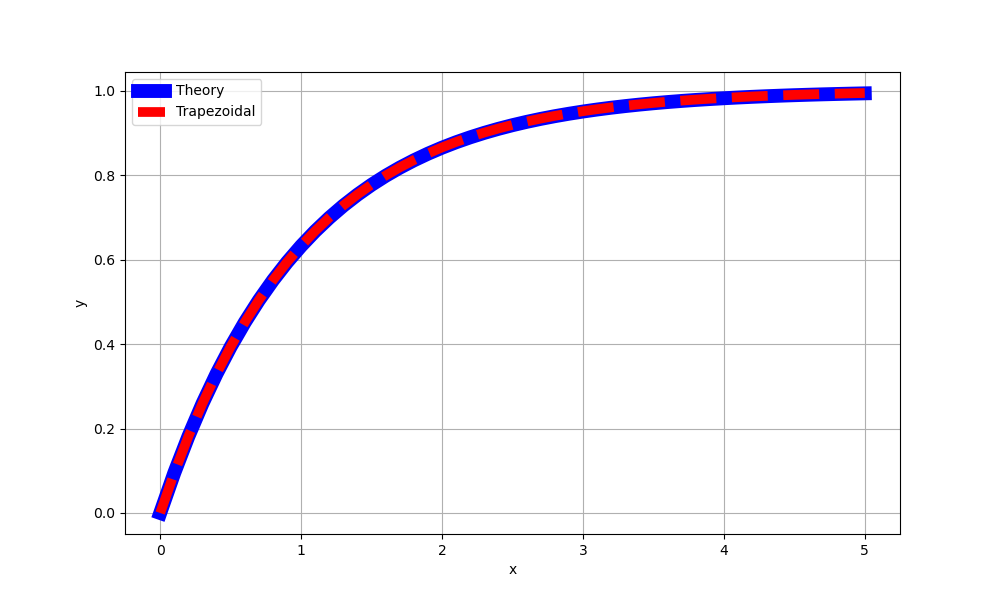
\includegraphics[width=0.7\columnwidth]{figs/Q2.png}
    \label{stemplot}
\end{figure}
\end{frame}

\end{document}
